\documentclass{config}
\usepackage[T1]{fontenc}
\usepackage[utf8]{inputenc}
\usepackage{graphicx}
\usepackage{color}
\usepackage{siunitx}
\usepackage{listings}
\usepackage{wrapfig}
\usepackage{subcaption}
\usepackage{float}
\usepackage[toc,page]{appendix} 
\usepackage{amsmath}
\usepackage{bigints}

\usepackage[labelfont=sc]{caption}
\title{Hyperelastic arteries}
%\author{Jeanne VENTRE}

%\instlabel{}{Master 2 of Engineering in Fluid Mechanics Fundamentals and Applications, Pierre and Marie Curie University (UPMC)}

\begin{document}

\maketitle
\section{1D equations}
  
Blood flows  in large arteries can be described by a set of reduced 1D equations resulting from integration of the reduced Navier-Stokes-Prandtl equations over a cross-section of artery. 

\begin{equation}\label{1D_system}
\left\{\begin{array}{rl}
\displaystyle \frac{\partial A}{ \partial t } + \frac{\partial Q}{\partial x} = & 0 \\ 
\displaystyle \frac{\partial Q}{\partial t} + \frac{\partial }{\partial x} \left( \frac{Q^2}{A}\right) + \frac{A}{\rho} \frac{\partial p }{\partial x} =&  \displaystyle - C_f \frac{Q}{A} \\
\end{array} \right.
\end{equation}

The objective of this report is to study several laws for the pressure gradient that appears in system (\ref{1D_system}) which accounts for fluid structure interactions. \\

To describe the artery wall, we assume that deformations and displacements are small. Under the hypothesis that there is no axial deformation such that the stretch in the $x$ direction is approximately equal to 1 (i.e $\lambda_2 \approx 1 $). Finally, assuming that the thickness of the wall is small compared to the radius of the artery leads to neglecting the deformation in the radial direction (i.e. $\sigma_3 = 0$). Only the stress in the tangential direction remains. We explore three different laws for the arterial wall: Sec \ref{sec_elastic} shows the example of to an elastic law for the pressure gradient, Sec \ref{sec_Varga} corresponds to Varga's law and finally Sec. \ref{sec_NeoHooke} for Neo-Hooke's law. In the final section, the analytic solution of system \ref{1D_system} with a specific pressure law is given. Comparison with the numerical solution is shown and plots of the error are given. \\ 

The figure below shows qualitative shape of the stress as a function of the strech $\lambda_1 = R/r_0$ ($r_0$ being the reference radius) for the three laws that we investigate. 

\begin{figure}[H]
\begin{center}
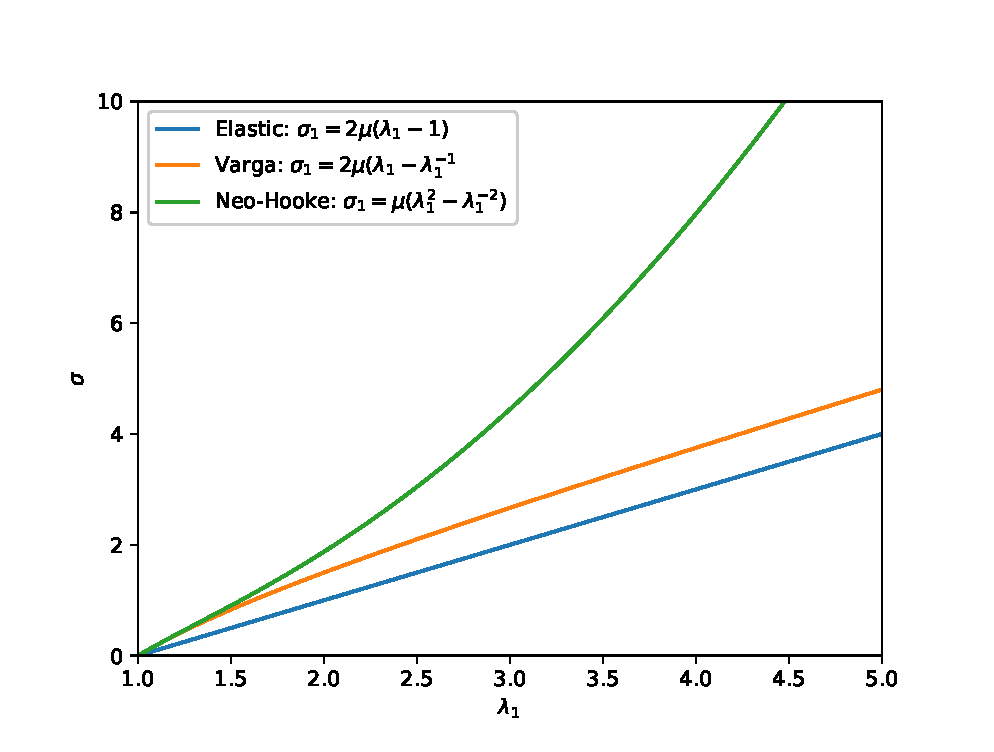
\includegraphics[scale=0.6]{figures/sigma.eps}
\caption{Stress as a function of strech for different laws.}
\label{sigma_lambda}
\end{center}
\end{figure}

The relation between the tangential stress and the pressure jump over the wall is described by the following equation:

\begin{equation}\label{pressure_relation}
p - p_{ext}= 2 \frac{h_0}{r_0} \frac{\sigma_1}{\lambda_1 ^2}
\end{equation}

where $h_0$ is the reference arterial wall thickness and $\sigma_1$ the principal stress in the tangential direction. \\ 

This pressure is plotted against the cross-sectionnal area for several stress laws (described in more details later) on the figure below.

\begin{figure}[H]
\begin{center}
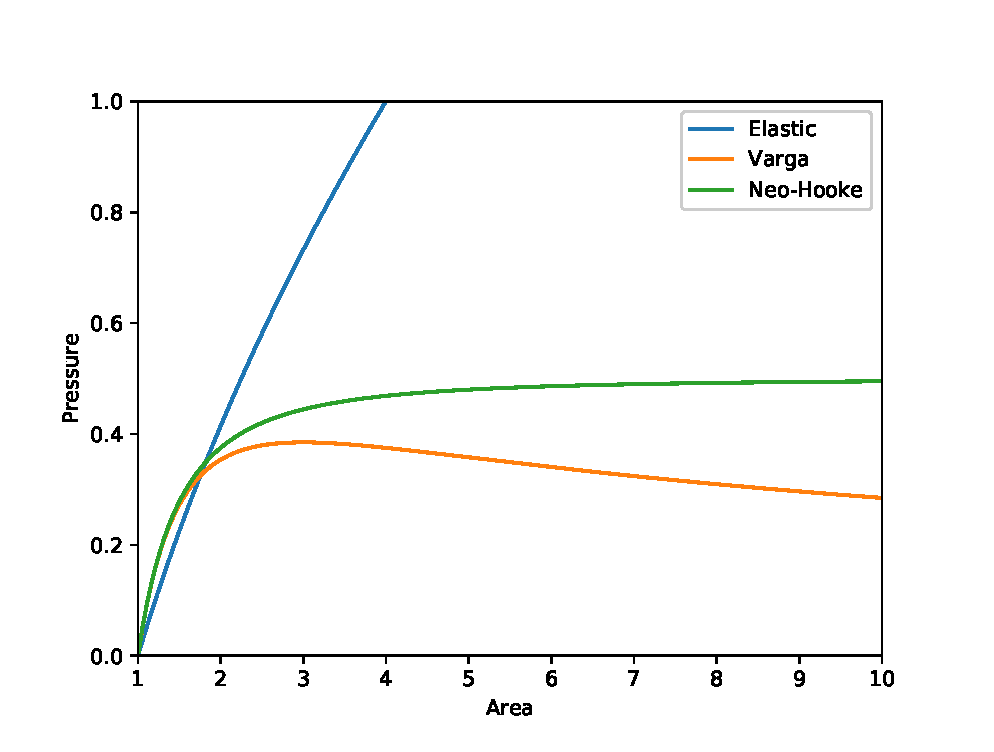
\includegraphics[scale=0.6]{figures/p_A.eps}
\caption{Pressure as a function of area for different laws.}
\label{p_A}
\end{center}
\end{figure}

The elastic wave speed in large arteries is assumed to be of the following form:

\begin{equation}\label{def_c}
c = \sqrt{\frac{A}{\rho} \frac{\partial p}{\partial A}}
\end{equation} 

On the figure below, we plotted the wave speed for each of the laws investigated in what follows. 

\begin{figure}[H]
\begin{center}
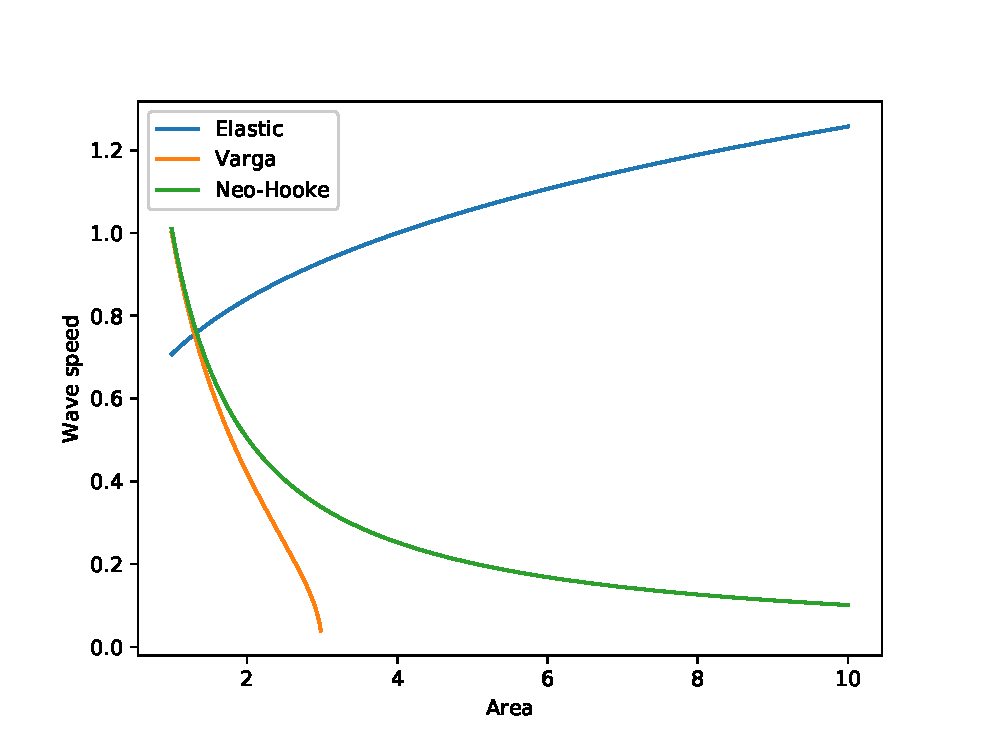
\includegraphics[scale=0.6]{figures/c_A.eps}
\caption{Wave speed $c$ as a function of area for different laws.}
\label{c_a}
\end{center}
\end{figure}

%Elastic law from Fig. \ref{sigma_lambda} and \ref{p_A} corresponds to Sec. \ref{sec_elastic}, Varga's law corresponds to Sec. \ref{sec_Varga} and Neo-Hookean law corresponds to Sec. \ref{sec_NeoHooke}. \\ 

%\section{Linear law in $A$}\label{sec_linear}
%
%\begin{equation}
%p - p_{ext} =  K \left(A - A_0\right)
%\end{equation}
%
%\subsection{Calculation of wave speed}
%
%\begin{equation}
%c = \sqrt{\frac{K A}{\rho }}
%\end{equation}
%
%\subsection{Calculation of pressure gradient}
%
%\begin{equation}
%\frac{A}{\rho } \frac{\partial p}{\partial x} = \frac{\partial }{\partial x}\left( \frac{K}{2 \rho} A^2 \right)
%\end{equation}
%

\section{Elastic}\label{sec_elastic}

\begin{equation}\label{sigma_elastic}
\sigma_1 = 2 \mu (\lambda_1 -1) 
\end{equation}

with $\lambda_1 = R/r_0 $ the strech in the radial direction, $\mu = \displaystyle \frac{E}{2(1- \nu^2)}$,  $E$ Young's modulus and $\nu$ the Poisson coefficient. \\

Injecting Eq. (\ref{sigma_elastic}) in (\ref{pressure_relation}), leads to:

\begin{equation}
p -p_{ext} = \frac{2h_0}{R^2} 2 \mu (R- r_0)
\end{equation}

then linearizing around $R=r_0$, with $A = \pi R^2$ gives:

\begin{equation}
p- p_{ext} = \frac{2 h_0 2 \mu \sqrt{\pi}}{A_0} \left(\sqrt{A} - \sqrt{A_0}\right)
\end{equation}

Let us define $ \displaystyle K =  \frac{2 h_0 2 \mu \sqrt{\pi}}{A_0}$, which leads to:

\begin{equation}\label{pressure_elastique}
p- p_{ext} = K \left( \sqrt{A}- \sqrt{A_0}\right)
\end{equation}

\subsection{Calculation of wave speed}

Using the pressure relation from Eq. (\ref{pressure_elastique}) to calculate the wave speed from Eq. (\ref{def_c}), we obtain:
 
 \begin{equation}\label{c_elastique}
 c = \sqrt{ \frac{K}{2 \rho}\sqrt{A}}
 \end{equation}
 
\subsection{Calculation of pressure gradient}

\begin{equation}
\displaystyle \frac{A}{\rho} \frac{\partial p}{\partial x} = \frac{K \sqrt{A}}{2 \rho}\frac{\partial{A}}{\partial{x}}  = \frac{K}{3 \rho} \frac{\partial}{\partial x} \left( A^{3/2} \right) 
\end{equation} 

 
 System (\ref{1D_system}) becomes: 
 
\begin{equation}\left\{
\begin{array}{rl}
\displaystyle \frac{\partial A}{\partial t} + \frac{\partial Q}{\partial x} = & \displaystyle  0 \\
\displaystyle \frac{\partial Q}{\partial t} + \frac{\partial }{\partial x} \left( \frac{Q^2}{A} + \frac{K}{3\rho} A^{3/2} \right) = & \displaystyle - C_f \frac{Q}{A} 
\end{array}\right.
\end{equation} 


\begin{figure}[H]
   \begin{minipage}[c]{.46\linewidth}
     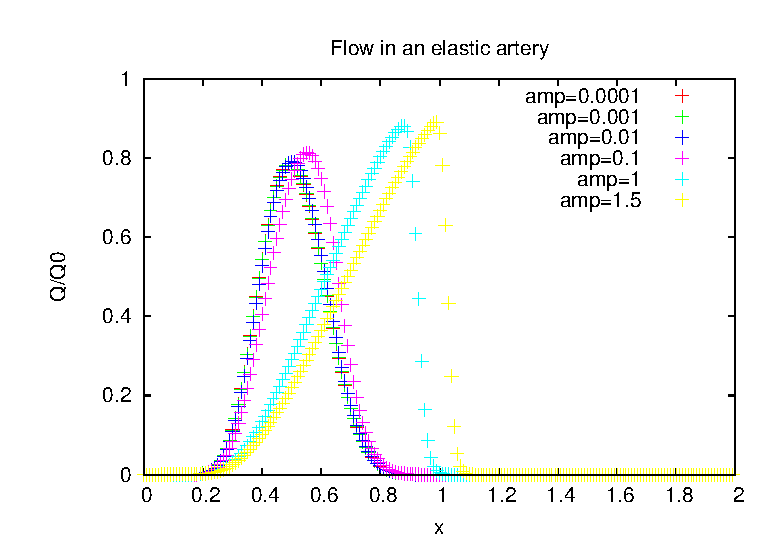
\includegraphics[scale=0.7]{figures/Q_elt1.eps}
   \end{minipage} \hfill
   \begin{minipage}[c]{.46\linewidth}
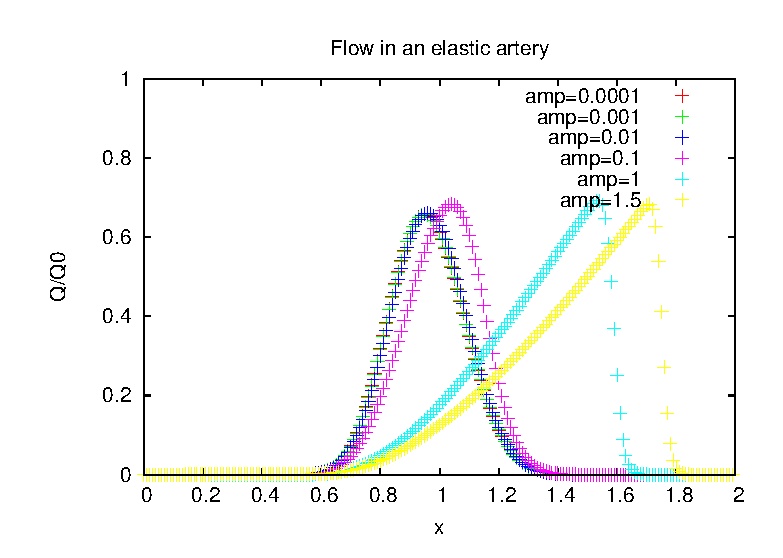
\includegraphics[scale=0.7]{figures/Q_elt2.eps}
   \end{minipage}
   \caption{Dimensionless flow rate in an elastic artery. Left: $t=0.96 s$, right: $t=1.6s$. N.B: "amp" is $Q_0$.}
   \label{Q_elastic}
\end{figure}

The figures on the above represent the dimensionless flow rate in an elastic artery with pressure law from Eq. (\ref{pressure_elastique}) at two times when varying the amplitude $Q_0$ of input at $x=0$, using Rusanov to compute the flux. 

\section{Varga}\label{sec_Varga}

Following the same steps as in Sec. \ref{sec_elastic}:

\begin{equation}\label{sigma_Varga}
\sigma_1 = 2 \mu (\lambda_1 - \lambda_1^{-1})
\end{equation}

Injecting Eq. (\ref{sigma_Varga}) in (\ref{pressure_relation}) gives:

\begin{equation}
p - p _{ext} = \frac{2 h_0}{r_0} \frac{r_0^2}{R^2 }\left(\frac{R}{r_0} - \frac{r_0}{R}\right)
\end{equation}

Assuming that this law is valid for large deformations allows us not to linearize around $R=r_0$. Then, using $A = \pi R^2$  and $A_0 = \pi r_0^2$ leads to:

\begin{equation}\label{p_final}
p - p_{ext} = 2 h_0 2 \mu \sqrt{\pi} \left( \frac{1}{\sqrt{A}} - \frac{A_0}{A \sqrt{A}}\right)
\end{equation}

Let us define $K' = \displaystyle 2 h_0 2 \mu \sqrt{\pi}$ which gives: 

\begin{equation}\label{pressure_varga}
p-p_{ext} = K' \left(\frac{1}{\sqrt{A}} - \frac{A_0}{A \sqrt{A}}\right)
\end{equation}

\subsection{Calculation of wave speed $c$}

\begin{equation}
c = \sqrt{\frac{K'}{\rho} \left(- \frac{1}{2 \sqrt{A} }+ \frac{3 A_0}{2} \frac{1}{A \sqrt{A}} \right)}
\end{equation}

\subsection{Calculation of pressure gradient }

\begin{align}
\displaystyle \frac{A}{\rho} \frac{\partial p}{\partial x} & =  \frac{K'}{\rho} \left(- \frac{1}{2 \sqrt{A} }\frac{\partial A}{\partial x}+ \frac{3 A_0}{2} \frac{1}{A \sqrt{A}} \frac{\partial A}{\partial x}\right) \\ 
&  = \frac{\partial }{\partial x}\left(- \frac{K'}{\rho} \sqrt{A} - 3 A_0\frac{K'}{\rho} \frac{1}{\sqrt{A}} \right)
\end{align}


System (\ref{1D_system}) becomes:

\begin{equation}\left\{
\begin{array}{rl}
\displaystyle \frac{\partial A}{\partial t} + \frac{\partial Q}{\partial x} = & \displaystyle  0 \\ 
\displaystyle \frac{\partial Q}{\partial t} + \frac{\partial }{\partial x} \left( \frac{Q^2}{A} - \frac{K'}{\rho} \sqrt{A} - 3 A_0 \frac{K'}{\rho} \frac{1}{\sqrt{A}} \right) = & \displaystyle - C_f \frac{Q}{A} 
\end{array}\right.
\end{equation}

\begin{figure}[H]
   \begin{minipage}[c]{.46\linewidth}
     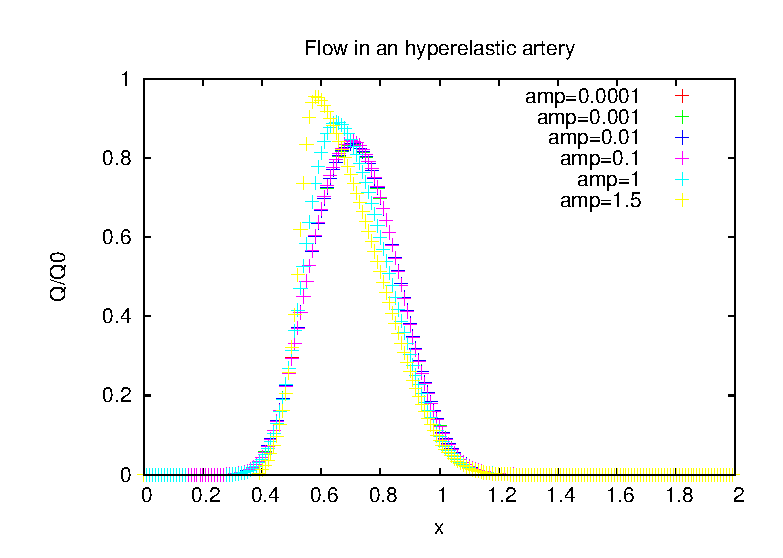
\includegraphics[scale=0.7]{figures/Q_vargat1.eps}
   \end{minipage} \hfill
   \begin{minipage}[c]{.46\linewidth}
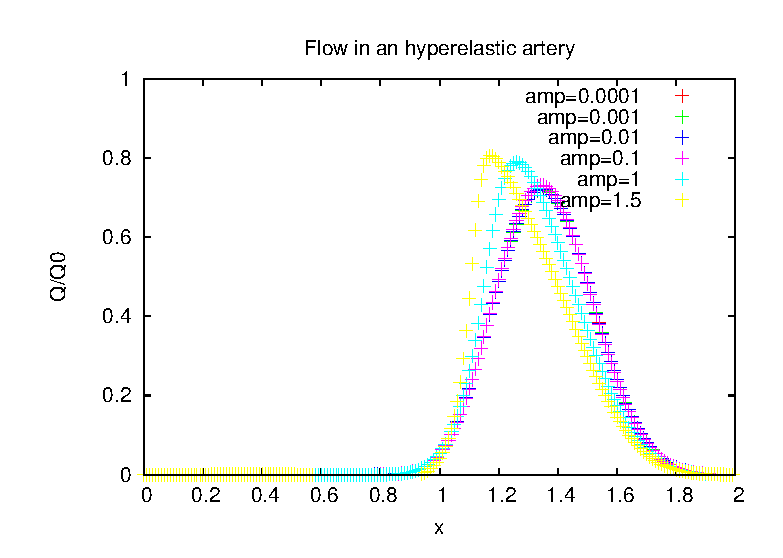
\includegraphics[scale=0.7]{figures/Q_vargat2.eps}
   \end{minipage}
   \caption{Dimensionless flow rate in an hyperelastic artery using Varga's law when varying the amplitude $Q_0$ of input at $x=0$ using Rusanov to compute the flux. Left: $t=0.96 s$, right: $t=1.6s$}
   \label{Q_varga}
\end{figure}


\section{Neo-Hooke}\label{sec_NeoHooke}

\begin{equation}\label{sigmaNH}
\sigma_1 = \mu (\lambda_1^2 - \lambda_1^{-2})
\end{equation}

\begin{equation}
p- p_{ext} = 2 \frac{h_0}{r_0} \mu \left(1 - \lambda_1 ^{-4} \right)
\end{equation}

\begin{equation}
p - p_{ext} = 2 h_0 \mu \frac{\sqrt{\pi}}{\sqrt{A_0}} \left(1 -\left( \frac{A_0}{A}\right)^2\right)
\end{equation}

Let us define $\displaystyle K'' = 2h_0 \mu \frac{\sqrt{\pi}}{\sqrt{A_0}} = K/2$: 

\begin{equation}
p-p_{ext} = K''  \left(1 -\left( \frac{A_0}{A}\right)^2\right)
\end{equation}

\subsection{Calculation of wave speed}

\begin{equation}
c = \sqrt{\frac{K}{\rho} \frac{A_0^2 }{A^2}}
\end{equation}

\subsection{Calculation of pressure gradient }

\begin{align}
\frac{A}{ \rho}\frac{\partial p}{\partial x} & = \frac{K A_0^2}{\rho} \frac{1}{A^2} \frac{\partial A}{\partial x} \\
& = \frac{K A_0^2}{\rho} \frac{\partial}{\partial x}\left(-\frac{1}{A} \right)
\end{align}

System (\ref{1D_system}) becomes:

\begin{equation}
\left\{ 
\begin{array}{rl}
\displaystyle \frac{\partial A}{\partial t} + \frac{\partial Q}{\partial x} = &\displaystyle  0 \\
\displaystyle \frac{\partial Q}{\partial t} + \frac{\partial }{\partial x} \left( \frac{Q^2}{A} - \frac{K}{\rho} \frac{A_0^2}{A} \right) =& \displaystyle  - C_f \frac{Q}{A} \\
\end{array}\right.
\end{equation}

\begin{figure}[H]
   \begin{minipage}[c]{.46\linewidth}
     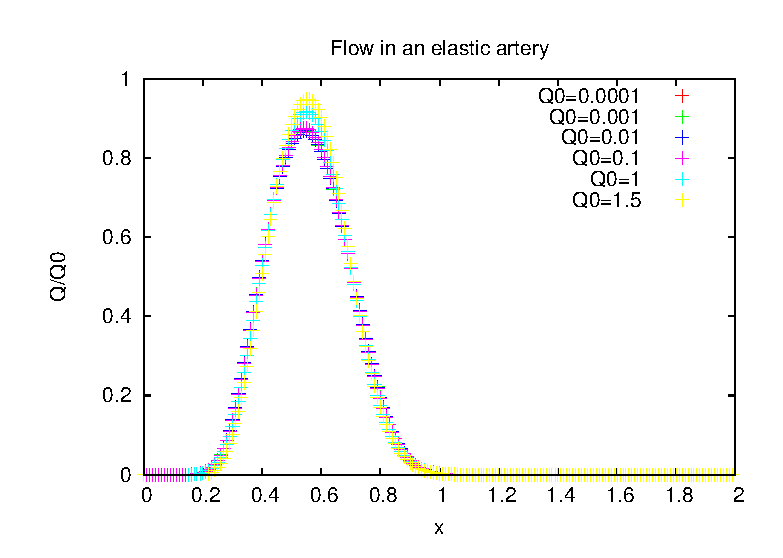
\includegraphics[scale=0.7]{figures/Q_NH_t1.eps}
   \end{minipage} \hfill
   \begin{minipage}[c]{.46\linewidth}
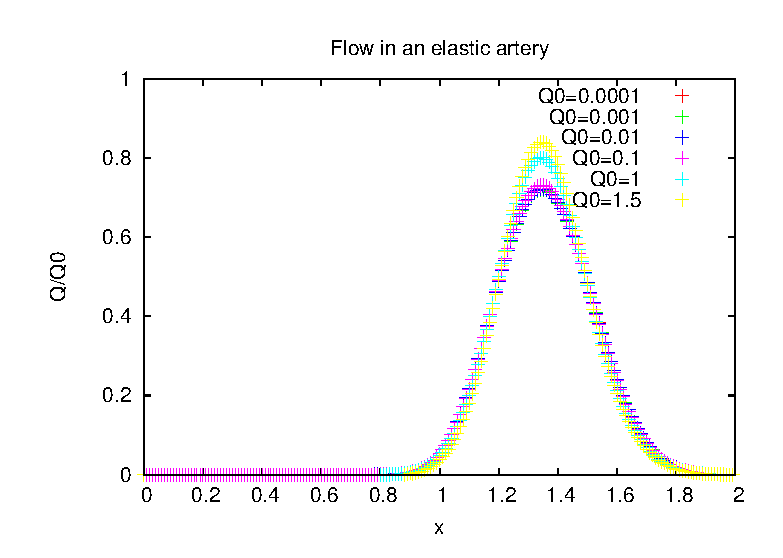
\includegraphics[scale=0.7]{figures/Q_NH_t2.eps}
   \end{minipage}
   \caption{Dimensionless flow rate in an hyperelastic artery using Neo-Hooke's law when varying the amplitude $Q_0$ of input at $x=0$ using Rusanov to compute the flux. Left: $t=0.96 s$, right: $t=1.6s$}
   \label{Q_NH}
\end{figure}

\section{Analytic solution}

In the case where $ p \propto A $, in the small amplitude approximation, system (\ref{1D_system}) has an analytic solution of the form:

\begin{equation}
Q =e^{i (k_r x - \omega t)} e^{-k_i x}
\end{equation}

where we impose at $x=0 $ that the flow is half of a sine with small amplitude and with $\omega$ the frequency, at $t=0$ the flow $Q$ is 0 and the area $A$ is 1.

\begin{figure}[H]
\begin{center}
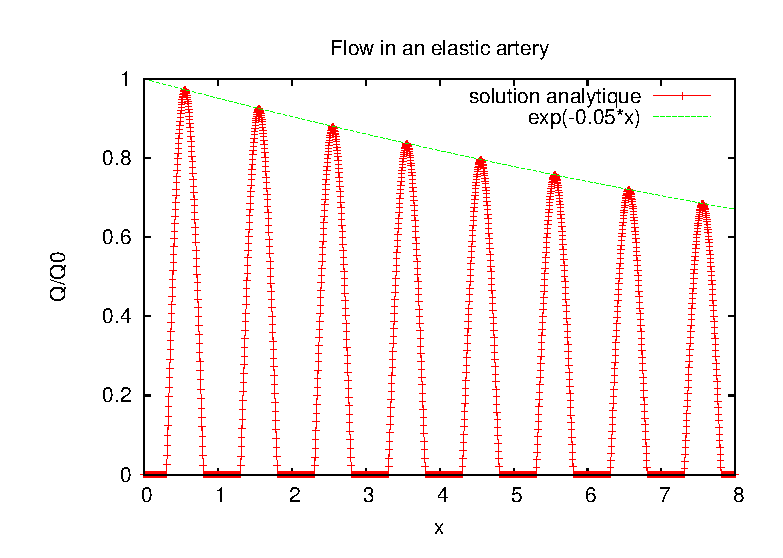
\includegraphics[scale=1]{figures/Q_analytic.eps}
\caption{Analytic solution with exponential decrease.}
\label{Q_analytic}
\end{center}
\end{figure}

The figure hereinabove shows the analytic solution of system (\ref{1D_system}), with a linear pressure with respect to cross-section $A$. The inlet is half of a sine to mimic cardiac impulse. This pulse propagates along the artery with an exponential decrease due to the friction term $\displaystyle -C_f \frac{Q}{A}$ that appears in the right hand side of the 1D equations.  \\ 

The figure below shows the error between the dimensionless analytic solution and the dimensionless numerical solution defined as:

\begin{equation}\label{def_error}
error =\sqrt{ \int (Q_{analytic} - Q )^2 \mathrm{d}x }
\end{equation}

We first investigate the effect of the space step on the numerical solution. The figure below shows a comparison of the analytic solution (red solid line) with the numerical solution for two numbers of space points Nx.

\begin{figure}[H]
\begin{center}
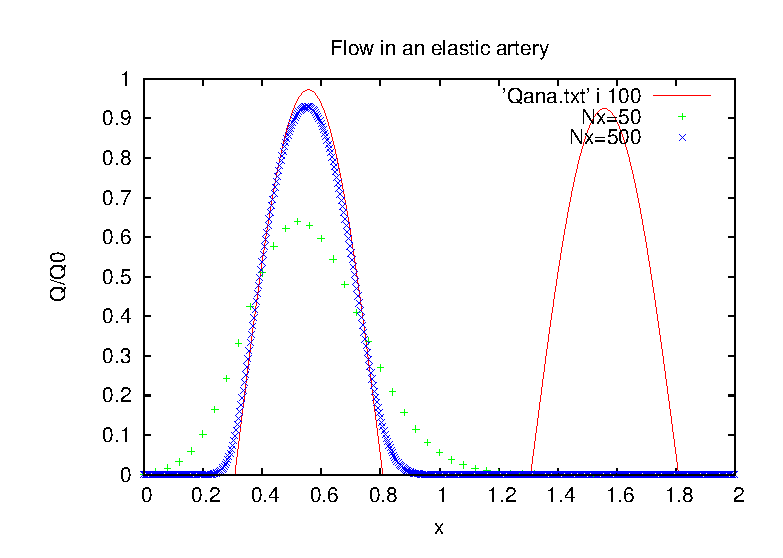
\includegraphics[scale=1]{figures/Q_Nx.eps}
\caption{Comparison between analytic and numerical solution of flow rate in an elastic artery for different number of space points.}
\label{Q_Nx}
\end{center}
\end{figure}

The figure on the above shows that quantitatively, the error described in (\ref{def_error}) highly decreases when the number of space iterations increases. \\

Now we plot in logscale the error defined previously in Eq. (\ref{def_error}) against the space step $\mathrm{dx}$.

\begin{figure}[H]
\begin{center}
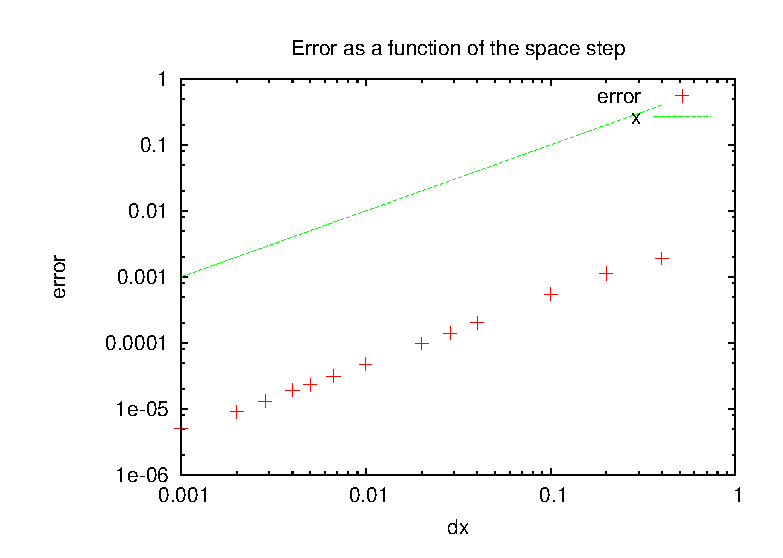
\includegraphics[scale=1]{figures/err_Nx.eps}
\caption{Integral of difference between analytic solution and numerical solution as a function of the number of space points Nx.}
\label{err_dx}
\end{center}
\end{figure}

The error scales in $\mathrm{dx}$ as the discretization scheme is of order 1. \\

Now we are insured of the order and convergence of the scheme, we can investigate the effect of the amplitude on the error defined in Eq. (\ref{def_error}).

\begin{figure}[H]
\begin{center}
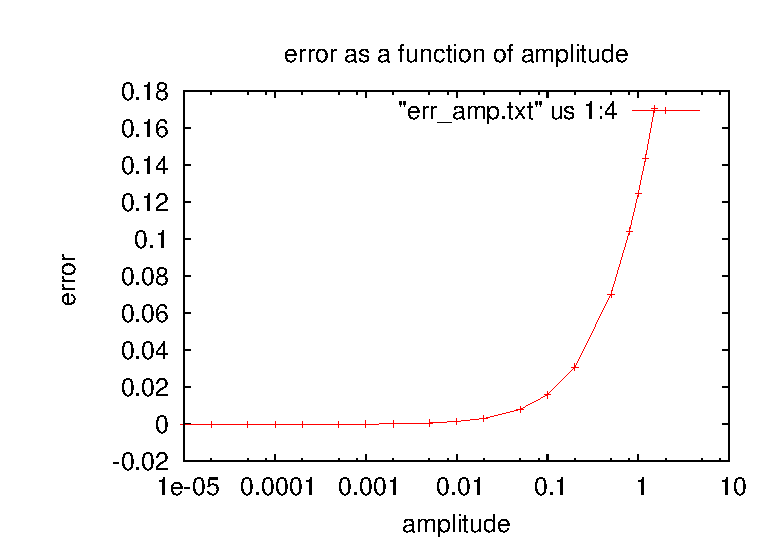
\includegraphics[scale=1]{figures/erreur_amplitude.eps}
\caption{Integral of difference between analytic solution and numerical solution as a function of amplitude $Q_0$.}
\label{err_amp}
\end{center}
\end{figure}

The error increases with respect to amplitude $Q_0$. It seems fairly logical since the analytic solution is only valid for small amplitudes of inlet flow rate. \\ 

\end{document}
